\documentclass[11pt]{article}
\usepackage[margin=1in]{geometry}
\usepackage{amsmath,amssymb,graphicx,booktabs}
\title{A Short-Time PINN Benchmark for Dysthe Equation (1.27)}
\author{}\date{Checkpoint: 17 September 2026}
\begin{document}\maketitle
\begin{abstract}
A physics-informed neural network trained for 20,000 steps reproduces an independent Fourier solution with a maximum sampled relative complex-field error of $0.6651\%$ on $0\le t\le0.5$. Peak error is $0.2148\%$ and integrated squared-magnitude drift is $0.1806\%$. The accompanying reference refinement screen passes. These results support one short-time periodic benchmark; seed robustness, long-time accuracy, decay exponents, and experimental validation remain unestablished.
\end{abstract}
\section{Problem and training}
The sole target is the full nonlinear equation (1.27) in \textit{Dysthe3D-2}:
\begin{equation}
iE_t+(1-i\epsilon_1\partial_z)(E_{xx}+E_{yy})-E_{zz}
-i\epsilon_2E_{zzz}+(1+i\epsilon_1\partial_z)(|E|^2E)=0.
\end{equation}
Here $E$ is a complex optical envelope, $t$ is normalized propagation distance, $x,y$ are transverse coordinates, and $z$ is retarded time. Envelope magnitude is not fluid velocity. The coefficients are $\epsilon_1=0.00831834509$ and $\epsilon_2=0.00498719622$.
On the periodic box $[-6,6)^3$, the synthetic initial condition is
\[
E(0,x,y,z)=0.3\prod_{q\in\{x,y,z\}}\left(\frac{1+\cos(2\pi q/12)}{2}\right)^3.
\]
The network has four hidden layers of width 64, tanh activations, three Fourier harmonics per coordinate, and two real outputs. The ansatz $E_\theta=E_0+(t/0.5)N_\theta$ imposes the initial condition exactly. Periodic input features impose periodicity of the field and its spatial derivatives.

Training uses float64 Adam, learning rate $3\times10^{-4}$, 512 resampled residual points per step, 512 fixed validation points, and seed 20260916. No reference solution samples enter training. This network learns one initial-value problem, not a family of inputs or an inverse estimate of the coefficients.
\section{Execution and evidence}
Training took 3584 seconds (59.7 minutes) on an NVIDIA A100-PCIE-40GB. Final training and validation residual MSEs were $1.2064\times10^{-7}$ and $1.5244\times10^{-7}$. Reported peak allocated GPU memory was $0.2134$ GiB; this excludes reserved memory and other process overhead and is not a measured total GPU footprint.

The review uses committed JSON metrics and rendered figures from commit \texttt{0af73b7}. Training records clean source revision \texttt{d2bda06}. Configurations and duplicated report metrics agree, and the evaluation reference path matches the audit recommendation. Raw checkpoint and field arrays were not included in this push; the field errors were therefore not independently recomputed in this review.
\clearpage
\section{Reference audit and measured accuracy}
The reference uses Fourier spatial differentiation, a strict cubic spectral cutoff, and integrating-factor RK4. The audit compares $32^3$ and $64^3$ grids at fixed periods, then halves the fine-grid step from $0.001$ to $0.0005$. Maximum relative field discrepancies are $2.541\times10^{-6}$ for spatial refinement and $3.233\times10^{-14}$ for time refinement. The latter is at roundoff scale and does not establish a measured convergence order. Maximum spatial-refinement peak discrepancy is $4.239\times10^{-6}$. These pass the provisional reference limits of $0.1\%$ field and $0.5\%$ peak disagreement, but are not rigorous error bounds.

At eleven saved times, the PINN is compared with the refined reference without phase alignment or amplitude renormalization. With $P=\max_{\rm grid}|E|$ and $M=\Delta V\sum_{\rm grid}|E|^2$, the diagnostics are
\[
e_E=\frac{\|E_\theta-E_r\|_2}{\|E_r\|_2},\qquad
 e_P=\frac{|P_\theta-P_r|}{P_r},\qquad
 e_M=\frac{|M_\theta-M_r|}{M_r}.
\]
\begin{center}\begin{tabular}{rrrr}\toprule
$t$ & $100e_E$ & $100e_P$ & $100e_M$\\\midrule
0.00 & 0.0000 & 0.0000 & 0.0000 \\
0.05 & 0.0923 & 0.0592 & 0.0320 \\
0.10 & 0.1591 & 0.0795 & 0.0481 \\
0.15 & 0.2164 & 0.0776 & 0.0571 \\
0.20 & 0.2733 & 0.0660 & 0.0662 \\
0.25 & 0.3330 & 0.0520 & 0.0801 \\
0.30 & 0.3954 & 0.0371 & 0.1007 \\
0.35 & 0.4597 & 0.0165 & 0.1267 \\
0.40 & 0.5254 & 0.0207 & 0.1534 \\
0.45 & 0.5929 & 0.0908 & 0.1741 \\
0.50 & 0.6651 & 0.2148 & 0.1806 \\
\bottomrule\end{tabular}\end{center}
\begin{center}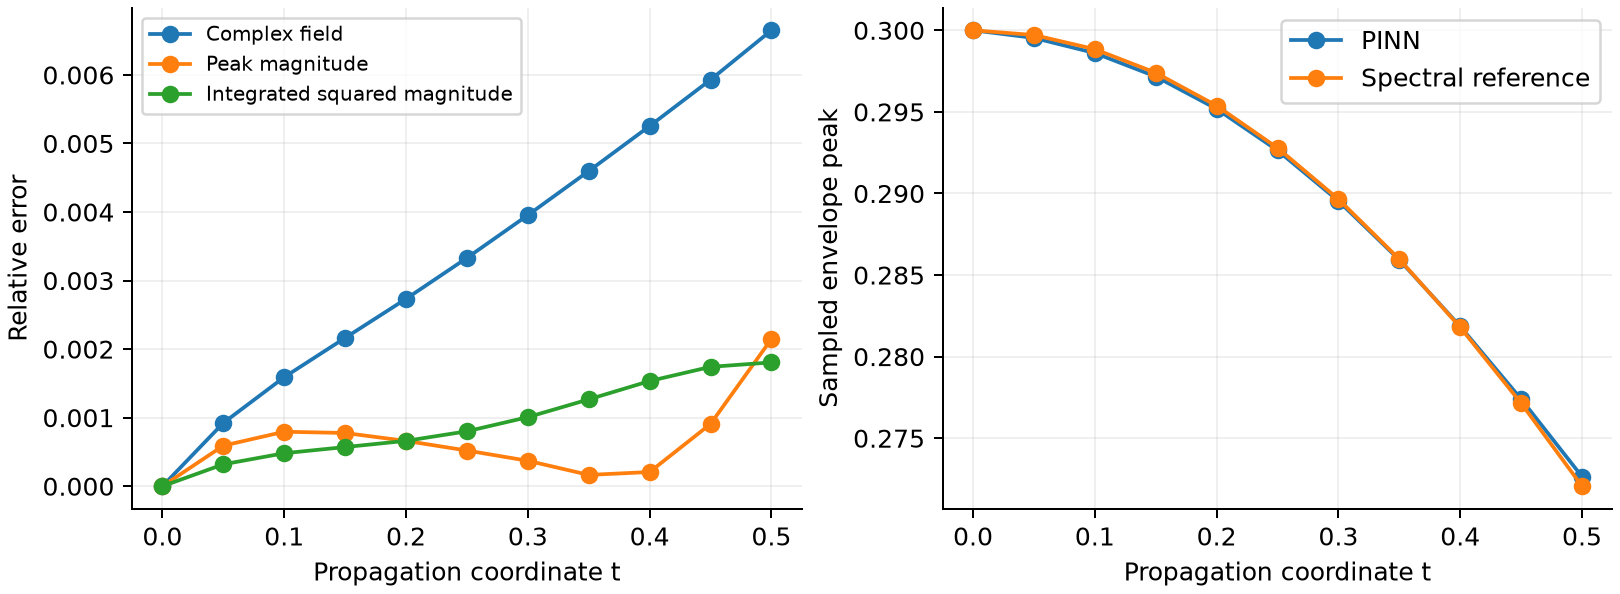
\includegraphics[width=\linewidth]{errors.png}\end{center}
\noindent\textbf{Figure 1.} Error growth and envelope peaks. The plotted errors are fractions: $0.00665$ means $0.665\%$. The peak curves nearly coincide, while complex-field error increases throughout the sampled interval.
\clearpage
\section{Spatial structure and interpretation}
\begin{center}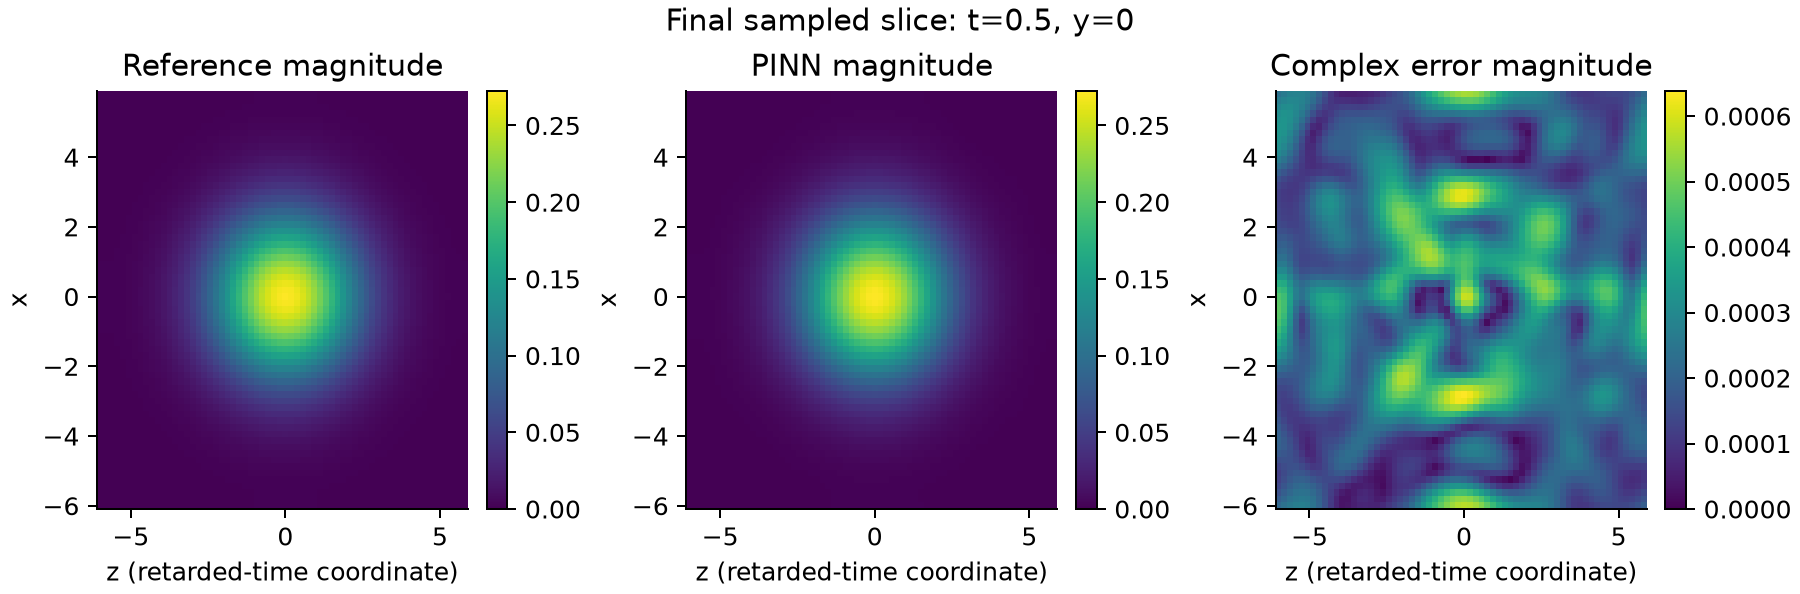
\includegraphics[width=\linewidth]{slices.png}\end{center}
\noindent\textbf{Figure 2.} Central $y=0$ slice at $t=0.5$. Reference and PINN magnitudes share a color scale. The error panel uses its own much smaller scale and includes phase disagreement; it is not a new physical wave. A single slice cannot summarize the full three-coordinate field, which is why the volumetric error is also reported.

The reference peak falls from $0.300000$ to $0.272057$, a $9.31\%$ decrease. Its integrated squared magnitude remains constant to about $1.07\times10^{-14}$ relative drift. This is consistent with redistribution of the envelope rather than loss of its integrated squared magnitude. The PINN predicts a final peak of $0.272642$ and loses about $0.181\%$ of that integral; this discrepancy is numerical error, not demonstrated physical dissipation.

The run satisfies the previously proposed per-run screens: maximum field error below $1\%$, peak error below $2\%$, and mass drift below $1\%$. However, the proposed minimum of three independent training seeds has not been met. Agreement is measured at the saved grid points and times, not certified everywhere between them. The increasing field error makes extrapolation beyond the training interval particularly unjustified.
\section{What follows for the decay question}
This calculation establishes a useful short-time accuracy baseline for the full nonlinear equation. It does not identify an asymptotic decay exponent. A decrease over $0\le t\le0.5$ cannot distinguish competing large-$t$ laws, and a periodic-box experiment cannot directly certify a whole-space dispersive inequality. Neither a soliton nor a counterexample to decay has been demonstrated.

The next experiment should repeat this unchanged benchmark with two additional seeds and compare the same diagnostics. After that screen passes, extend the propagation window incrementally and repeat reference refinement and accuracy checks on each window. Whole-space decay work additionally requires a fixed localized input consistently represented on expanding boxes; changing the period in the present initial formula also changes the packet width and would confound that comparison. Retain raw arrays and checkpoints so later reviews can recompute errors and examine phase and three-dimensional structure.

\paragraph{Reproducibility bundle.} The accompanying source archive includes this LaTeX file, the two submitted figures, evaluation metrics, reference audit, training summary, and training history. It preserves the recorded checkpoint and reference hashes in the JSON metadata.
\end{document}
